\documentclass[../main.tex]{subfiles}

\begin{document}

The root directory of the source code is "ITD". Inside of it there are three folders:

\begin{description}
	\item[ITD doc] Source code of this document.
	\item[TrackMeServer] Source code of the back-end server: Application Server Mobile Client, Application Server Data4Help, Database Server and Web Server components.
	\item[MobileApp] Source code of the mobile application and wearable module.
\end{description}

\subsection{TrackMeServer}

The four modules inside this directory all share the same basic structure: inside the component's directory (eg. ApplicationServerMobileClient) there is the main javascript file to be launched with node (eg. ApplicationServerMobileClient.js), the documentation source for the component if available (doc.yml), and a routes directory that futher defines funcionalities provided by the component.

The directory named "common" contains two files used by the components:

\begin{description}
	\item[config.json] Contains configuration variables that can or must be set for the components to work, and can be overridden by environment variables (see chapter 6).
	\item[common.js] Contains functions often used by all other components; they are defined here to avoid code repetition and ease the development process.
\end{description}

One more directory named "support" contains files useful for development and evaluation. Three python scripts and a standalone node (javascript) file. The python scripts are written and tested for python 3 version 3.7.2 and require the "requests" package:

\begin{description}
	\item[cleanDatabase.py] Simply performs a GET to /dropALL on the DatabaseServer component to reset the database tables (see the DatabaseServer component description below).
	\item[populateDatabase.py] This script uses the ApplicationServerMobileClient and ApplicationServerData4Help components to register random model data in the system.
	\item[subscriptionHandler.py] A simple server to listen and write data to simulate a company subscription's funcionality.
	\item[AmulanceDispatcherSimulator/dispatcher.js] Node JS server that simulates the external ambulance dispatcher simulator, required for AutomatedSOS funcionality.
\end{description}

Every main component javascript file sets up the environment and binds the service to the address provided by the config file (or environment variable).

\subsubsection{DatabaseServer}

This component has one more file, "knex.js", that sets up the connection with the DBMS.

Inside the main file the tables of the database are created, if they don't exists, then the files in "routes" are sourced for the various funcionalities. Also, a temporary endpoint is defined (GET to /dropALL), only for development and evaluation purposes, that can be used to drop all current tables and recreate them empty.

The three files in "routes" directory contain the endpoints relative to their name, for example "dbs\textunderscore user.js" contains all the endpoints to handle user informations.

\subsubsection{ApplicationServerMobileClient \& ApplicationServerData4Help}

As the DatabaseServer component, the main file set up the environment and binds the service to the provided address; these two components also provide an endpoint (GET to /docs) to the documentation of their API. Then they source the .js file in "routes" folder that contain the implementation of their endpoints funcionality.

The doc.yml is the source code of the documentation, read by swagger when starting the component through the swagger-jsdoc node module.

\subsubsection{WebServer}

The web server has a main file, WebServer.js, that set up the environments and configures an object useful to send emails named "trasporter" and the relative logic realized thanks to a Node.js module called "nodemailer".
In the folder "public" there are the html pages that the third party comapany will use, in particular "register.html", to register to the service with a form. The contents of the fields are checked with the javascript file "javascripts/validationForm.js" before sending the email.
The style of web pages is defined by a css file "stylesheets/style.css".

\subsection{MobileApp}
MobileApp is composed of two submodule, Flutter code and the android platform specific code.

\subsubsection{Flutter code}
as shown in Fig. 1, the structure of the code is pretty simple
\begin{description}
	\item[controllers] Contains the class channelController, responsible for platform specific methods invocation. In brevity, this class link Flutter code with Java code.
	\item[models] A modelization of the database classes, made easier to manage data received trough HTTP requests.
	\item[profileManager] As seen in the DD, this component will handle all the functionalities regarding the user, such as registration, login, registering a new Wearable device etc. This is where the main logic of the app is located
	\item[screens] This is were Flutter shines, those are the screens of the application, a collection of statefull and stateless widgets.
	\item[styles] files with useful font and theme that give a distinctive style to the application
	\item[utils] a collection on useful methods and class. CountryCodePicker is a custom version of the dart plugin while validators are the function used to verify the user form inputs.
\end{description}





	\begin{figure}[H]
		\centering
		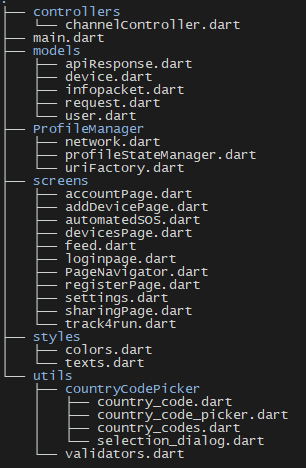
\includegraphics{tree_flutter.png}
		\caption{tree view for the lib folder}
		\label{fig:lib_tree.png}
	\end{figure}

\subsubsection{Platform specific code (Java)}
Is composed of two macro classes located in \\ "../MobileApp/TrackmeMobile/trackmemobile/android/app/src/main/java/com/trackme/trackmemobile"
\begin{description}
	\item[MainActivity.java] launch the application and contains a CommunicationPlugin class that handle the platform call made by Flutter.
	\item[InfoPacketHandler.java] handle the connection with the WearOS device, receive the infoPackets on a nonBlockingQueue of fixed size and dispatch the received infoPacket to the TrackMe mobile application server (Fig2)
\end{description}

\begin{figure}[H]
	\centering
	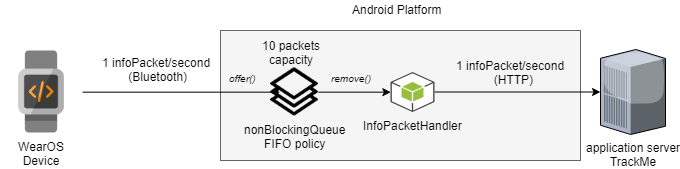
\includegraphics[width=\linewidth]{queue.png}
	\caption{infoPacket "cycle of life"}
	\label{fig:infopacketscycle.png}
\end{figure}

\subsubsection{TrackmeWear}

todo

\subsection{Notable algorithms}

The source code is commented and should not be difficult to follow and understand; however, there are some more elaborate portions for which could be useful a little explanation:

\begin{itemize}

	\item Filters for group requests, passed in the POST body, are parsed in groups: each group of filters has a number associated to it that goes after the filter's name, for example:

	 ageStart1=18\&ageEnd2=25\&street2=risorgimento

	 are two different groups, respectively group 1 and 2. Multiple filters can be specified per group, and if no number is specified it is assumed to be number 1. Each filter inside the group is in a logical AND relation with all the other filters in the same group, while the different groups are in logical OR relation with all the other groups. So, the example above would search for users that (are at least 18 years old) OR (are at most 25 years old AND live in risorgimento street).
	\item Subscriptions for authorized requests require that the company set a server capable of receiving data from TrackMe's server, sent as POST requests containing user's data in JSON format, and must respond to every request with status code 200 (an example of such server is provided in TrackMeServer/support/subscriptionHandler.py). It must provide a reachable link to such service when subscribing. If such server is not reachable or won't respond at the moment of subscribing, the operation will fail. If the subscription is succesfully activated, and the company's server then stops satisfying the above requirements, the subscription will be automatically deactivated.
	
\end{itemize}

\end{document}
